% Springer Nature sn-jnl v3.1, APA author-year. Anonymous reviewer copy.
\documentclass[pdflatex,sn-apa]{sn-jnl}
\usepackage{amsmath,amssymb}
\usepackage{longtable,booktabs,array}
\usepackage{graphicx}
\usepackage{calc}
\setcounter{secnumdepth}{3}
\providecommand{\tightlist}{\setlength{\itemsep}{0pt}\setlength{\parskip}{0pt}}
\providecommand{\pandocbounded}[1]{#1}

\begin{document}
\title[Source Replay for Mixed-Unlabeled Adaptation]{Source Replay for Mixed-Unlabeled Adaptation in Multivariate Time-Series Anomaly Detection: Benefits, Costs, and Task Dependence}
\author{\fnm{Anonymous} \sur{Authors}}
\affil{\orgname{Withheld for review}}
\abstract{Unlabeled adaptation can expose a time-series anomaly detector to changing normal behavior and to unrecognized anomalies. We compare four update policies on two public tasks, Secure Water Treatment (SWaT) and Pooled Server Metrics (PSM), with a common detector and fixed chronological splits. At a fixed update budget, replacing half of the target windows with earlier nominally normal source windows improves pointwise average precision over target-only updating in all three paired seeds per task, by a mean of 2.61 percentage points on SWaT and 1.59 on PSM. At model-specific empirical thresholds, replay reduces false-positive counts on both tasks, while alarm coverage after three-point confirmation increases on SWaT and decreases on PSM. All 512 selected PSM calibration points are attack-labeled, so the thresholds do not certify a normal false-alarm rate. A second comparison uses fit labels to assign abnormal or nominally normal donor windows to matched exposure slots before unlabeled learning. On SWaT, replay attenuates losses in average precision and coverage under this fixed intervention, with the same number of matched events. Neither arm shows an average-precision loss from abnormal versus normal replacement on PSM. The controlled comparisons identify when an established replay policy improves ranking and when that improvement comes with lower event coverage.}
\keywords{Source replay, Mixed-unlabeled adaptation, Multivariate time-series anomaly detection, Contaminated training data, Empirical evaluation}
\maketitle
\section{Introduction}\label{introduction}

Anomaly detectors trained on a nominally normal record often encounter a
different mixture of operating states after deployment. Updating on a
later unlabeled record can help the detector accommodate new normal
behavior, but the same updates can change how it scores anomalies
present in that record. Whether adaptation helps therefore depends on
the outcome: a detector can rank abnormal points better across
thresholds and still cover less of a sustained episode at its calibrated
threshold.

Source replay presents earlier observations alongside new data and is
established in continual learning and adaptation
\citep{rolnick2019, buzzega2020, rostami2021}. Comparing replay with a
frozen detector combines the effects of more optimization, exposure to
the target record, and renewed access to the source. Comparing replay
only with ordinary target updating under a naturally mixed record also
leaves the response to added abnormal exposure unresolved. Accounting
for ordinary window replacement requires a separate normal-donor
control.

We use the published LEFT detector \citep{left2026} with a fixed
source-initialized state for each of two public tasks, SWaT and PSM. The
main comparison holds the detector, initial state, update budget, and
evaluation protocol fixed. One contrast replaces the second target
half-batch with earlier source observations while sharing the first
target half-batch across arms. A separate intervention replaces fixed
slots in that shared half-batch with either abnormal or nominally normal
windows from each task's authorized target-fit interval. The
replacements are matched by slot. Learning uses only numerical
observations.

The analysis asks three questions.

\begin{enumerate}
\def\labelenumi{\arabic{enumi}.}
\tightlist
\item
  Does ordinary mixed-unlabeled target updating improve detection
  relative to a frozen initialization or to continued source-only
  training?
\item
  Does source replay improve detection relative to a target-only update
  with the same total number of window presentations, and does the
  effect repeat across adaptation seeds?
\item
  Does the response to additional abnormal exposure differ from the
  response to a normal replacement, and does replay change that
  difference consistently across tasks?
\end{enumerate}

We make three empirical contributions.

\begin{enumerate}
\def\labelenumi{\arabic{enumi}.}
\tightlist
\item
  We define a matched four-arm comparison with explicit source and
  target access, optimization budgets, and calibration.
\item
  We document which benefits repeat across three paired seeds in SWaT
  and PSM, including cases where ranking, false alarms, event discovery,
  and sustained coverage disagree.
\item
  We use matched abnormal and normal replacements to characterize the
  limits of replay under added abnormal exposure.
\end{enumerate}

The contribution is empirical evidence about a fixed update policy. The
two task-specific initializations and chronological evaluation axes
bound what the comparisons establish. SWaT and PSM provide two settings
for studying differences in response, with three adaptation seeds for
describing variability within each setting.

\section{Related Work}\label{related-work}

\textbf{Multivariate anomaly detection.} Reconstruction and consistency
detectors infer abnormality from deviations from learned regularity.
LEFT represents temporal, spectral, and multiscale views and scores
disagreement through its published reconstruction pipeline
\citep{left2026}. TimeRadar instead learns a fractional time-frequency
domain and uses masked reconstruction and contextual deviation
objectives \citep{timeradar2026}. Its pretraining includes synthetic
anomaly information. Both supply mature detectors for studying update
policies. Their original training permissions and scoring context differ
from the mixed-unlabeled adaptation setting studied here. We use LEFT as
the shared detector in the primary comparisons and keep TimeRadar as a
separately identified external reference.

\textbf{Adaptation with unlabeled target observations.} M2N2 estimates a
trend and updates its reconstruction model on predicted-normal time
points within target windows \citep{m2n22024}. CANDI selects potential
false positives using anomaly scores and latent similarity, then applies
lightweight spatiotemporal adaptation \citep{candi2026}. These methods
address the risk of adapting to unreliable target samples and can update
as test observations arrive in their original settings. Source replay
draws earlier nominally normal observations and samples target windows
uniformly. Our CANDI reference adapts on the authorized target-fit
prefix and freezes before query scoring, so its results need to be
interpreted under that schedule.

\textbf{Anomaly contamination and experience replay.} TSAD-C learns from
contaminated training data using conditional diffusion for
decontamination and subsequent spatiotemporal dependency modeling
\citep{tsadc2025}. RoCA uses model-generated evidence about possible
outliers in a joint one-class and contrastive learning framework
\citep{roca2026}. Angel or Devil studies a related ambiguity: hard
normal samples and contaminating anomalies can have similar losses. Its
PLDA method combines the loss with a measure of parameter response to
small perturbations, then augments the training set iteratively
\citep{zhang2026plda}. Our replay arm uses a specified source pool and
uniform sampling, without a learned detector for contamination or
difficult normal samples. Earlier replay work includes behavioral
cloning in continual reinforcement learning, logit distillation, and
replay from a learned distribution for continual domain adaptation
\citep{rolnick2019, buzzega2020, rostami2021}. The matched experiments
here study the effect of substituting source windows at an equal update
budget and the response to extra abnormal exposure at fixed replacement
slots.

\textbf{Evaluation of temporal anomalies.} TSB-AD examines inconsistent
evaluation protocols and metric choices \citep{tsbad2024}. Xu and
Bostr\"{o}m identify benchmark modifications, leakage, and underspecified
baselines as reproducibility problems in time-series anomaly detection
\citep{xu2026methodology}. Volume-under-the-surface measures summarize
discrimination with range tolerance \citep{vus2025}. In our comparison,
rank measures use a fixed scored axis, and a separate calibration rule
defines alarms. We report one-to-one matched events, any overlap, and
the share of an event covered. These distinctions matter when score
distributions differ across models or a single alarm fragment overlaps
several events.

\section{Problem Formulation and Experimental
Protocol}\label{problem-formulation-and-experimental-protocol}

\subsection{Data roles and task scope}\label{data-roles-and-task-scope}

For a task, let \(x_t\in\mathbb{R}^d\) be its multivariate observations
and \(y_t\in\{0,1\}\) its point annotations where available. A nominally
normal source prefix supplies a source fit interval and a source
validation interval. A later target fit interval supplies unlabeled
observations for adaptation. We reserve separate chronological
calibration and query intervals. A \emph{task} is the combination of a
dataset, one fixed initial detector, and this assignment of data roles.
SWaT is a public water-treatment benchmark and PSM is an eBay
server-monitoring benchmark \citep{swat2016, psm2021}. We use the
archived 31-channel SWaT and 25-channel PSM representations. Each task
uses its own initial state. No data or weights are transferred between
SWaT and PSM.

Table 1 presents fixed chronological intervals.

\begin{longtable}[]{@{}
  >{\raggedright\arraybackslash}p{(\linewidth - 10\tabcolsep) * \real{0.1667}}
  >{\raggedright\arraybackslash}p{(\linewidth - 10\tabcolsep) * \real{0.1667}}
  >{\raggedright\arraybackslash}p{(\linewidth - 10\tabcolsep) * \real{0.1667}}
  >{\raggedright\arraybackslash}p{(\linewidth - 10\tabcolsep) * \real{0.1667}}
  >{\raggedright\arraybackslash}p{(\linewidth - 10\tabcolsep) * \real{0.1667}}
  >{\raggedleft\arraybackslash}p{(\linewidth - 10\tabcolsep) * \real{0.1667}}@{}}
\caption{Fixed chronological intervals. Ranges are half-open. Source
coordinates refer to the released training prefix. SWaT target
coordinates refer to the combined timeline and PSM target coordinates
refer to the released test record. The scored query axis retains only
positions covered by complete legal windows. Frozen window alignments,
channels, calibration point selection, and excluded tails are documented
in Appendix A.}\tabularnewline
\toprule\noalign{}
\begin{minipage}[b]{\linewidth}\raggedright
Task
\end{minipage} & \begin{minipage}[b]{\linewidth}\raggedright
Source fit / validation
\end{minipage} & \begin{minipage}[b]{\linewidth}\raggedright
Target fit
\end{minipage} & \begin{minipage}[b]{\linewidth}\raggedright
Calibration role
\end{minipage} & \begin{minipage}[b]{\linewidth}\raggedright
Query score axis
\end{minipage} & \begin{minipage}[b]{\linewidth}\raggedleft
Points / complete events
\end{minipage} \\
\midrule\noalign{}
\endfirsthead
\toprule\noalign{}
\begin{minipage}[b]{\linewidth}\raggedright
Task
\end{minipage} & \begin{minipage}[b]{\linewidth}\raggedright
Source fit / validation
\end{minipage} & \begin{minipage}[b]{\linewidth}\raggedright
Target fit
\end{minipage} & \begin{minipage}[b]{\linewidth}\raggedright
Calibration role
\end{minipage} & \begin{minipage}[b]{\linewidth}\raggedright
Query score axis
\end{minipage} & \begin{minipage}[b]{\linewidth}\raggedleft
Points / complete events
\end{minipage} \\
\midrule\noalign{}
\endhead
\bottomrule\noalign{}
\endlastfoot
SWaT & {[}0, 396000) / {[}396000, 495000) & {[}495000, 585000) &
{[}585544, 607479) & {[}608535, 944856) & 336,321 / 22 \\
PSM & {[}0, 105984) / {[}105984, 132481) & {[}0, 17568) & {[}18112,
21960) & {[}22656, 87744) & 65,088 / 48 \\
\end{longtable}

The LEFT scaler uses the entire released source prefix under its native
protocol, including the source validation observations. The source
half-batch draws from the source fit interval only. Every arm starts
from the same task-specific source-validation-selected checkpoint,
scaler, prototype state, and archived scoring step. The scaler stays
fixed during adaptation. Target query labels are opened for evaluation
after scoring. In the natural condition the learner receives no anomaly
labels. In the controlled condition fit labels belong to the separate
data-construction step in Section 5. Appendix A records the code
version, the raw roles, and the distinction between legal window support
and the final scored crop.

\subsection{Matched update policies}\label{matched-update-policies}

Write \(T\) and \(T'\) for target draws, and \(S\) and \(S'\) for source
draws. At each update, each draw contains 128 legal windows of length
192. The primed draws use separate, uniform random streams. Table 2 summarizes the four policies.

\begin{longtable}[]{@{}
  >{\raggedright\arraybackslash}p{(\linewidth - 4\tabcolsep) * \real{0.3333}}
  >{\raggedright\arraybackslash}p{(\linewidth - 4\tabcolsep) * \real{0.3333}}
  >{\raggedright\arraybackslash}p{(\linewidth - 4\tabcolsep) * \real{0.3333}}@{}}
\caption{Matched update policies. Each updated half-batch contains 128 legal windows.}\tabularnewline
\toprule\noalign{}
\begin{minipage}[b]{\linewidth}\raggedright
Policy
\end{minipage} & \begin{minipage}[b]{\linewidth}\raggedright
Update batch
\end{minipage} & \begin{minipage}[b]{\linewidth}\raggedright
Interpretation
\end{minipage} \\
\midrule\noalign{}
\endhead
\bottomrule\noalign{}
\endlastfoot
noU & None & The single frozen starting model for a task \\
TT & \([T,T']\) & Ordinary adaptation drawn entirely from the mixed
target fit interval \\
SS & \([S',S]\) & Continued optimization on the nominally normal source
fit interval \\
R & \([T,S]\) & Equal-share source replay during mixed-unlabeled
adaptation \\
\end{longtable}

TT and R share the exact first-half target draw \(T\) within a seed. SS
and R share the exact second-half source draw \(S\). All updating arms
train all LEFT parameters with a fresh Adam optimizer at learning rate
\(10^{-4}\). Each update uses batch size 256, one native forward and
state update, and the original LEFT loss on the full batch. We evaluate
the checkpoint after exactly 2,000 optimizer updates. Seeds 2025, 2026,
and 2027 define matched draws and training randomness. R\ensuremath{-}TT measures the
effect of replacing \(T'\) with \(S\) at matched update and
window-presentation budgets. The comparison combines additional source
exposure and fewer target presentations. SS measures continued
source-only training on the original source observations. The earlier
batch-128 ordinary U run remains a separate historical reference.

All primary adaptation runs use the same per-arm budgets above. Appendix
B lists archived A40 occupancy by execution phase, separating
source-initialization, adaptation/readout, and reused assets. The timing
records measure historical GPU occupancy and do not establish
standardized cross-model speed.

\subsection{Readout, calibration, and event
definitions}\label{readout-calibration-and-event-definitions}

The primary detector emits native scores at all positions within
aligned, nonoverlapping windows of length 192. A score is available only
at the end of its window. The resulting analysis is offline and
retrospective, and a score at a position can depend on later
observations in the same window. Windows used for scoring stay inside
their authorized roles. Each fitted model uses its own scores at the
same 512 calibration locations. The threshold is the empirical 0.99
quantile with the higher convention. Strict alarms use
\(a_t=\mathbf{1}[s_t>\tau]\), and three-point confirmed alarms use
\(c_t=a_t a_{t-1}a_{t-2}\) on consecutive scored points without
backfilling. Confirmation restarts at discontinuities. There are 38
attack-labeled points in the 512 SWaT calibration locations and 512 in
PSM. These are post hoc label counts on fixed locations. The calibration
rule sets an empirical mixed-data operating point and does not establish
an equal or certified normal false-alarm budget. PSM's ranking measures
remain evaluable independently of this operating point.

We report unadjusted average precision (AP), ROC-AUC, and VUS-PR and
VUS-ROC using the archived LEFT range implementation
(\texttt{windowSize=100}, \texttt{thre=250}) \citep{vus2025}. AP denotes
the stepwise precision-recall average rather than trapezoidal area.
Point recall and false-positive counts use the full scored query axis.
Event statistics use complete events only. In PSM, observed points from
two boundary-truncated events remain in the pointwise ranking and point
metrics. A complete event is an \emph{any-hit} event if it overlaps at
least one alarm. A separate chronological first-unmatched-overlap rule
assigns at most one alarm fragment to each event and at most one event
to each fragment. The reported matched count, precision, recall, and F1
use this rule. It is not maximum matching.

Complete-event point coverage pools the alarmed points over the total
duration of the complete eligible events. For events longer than 512
samples, we measure steady coverage starting at event onset plus 512. We
present the mean of per-event steady coverages and the pooled proportion
of steady event points. They answer different questions when event
lengths vary substantially. The archived tables retain longest missed
spans, normal alarm fragments, matched and any-hit counts, and separate
retrospective location and availability offsets. Offset medians use hits
only. The tables record right-censored events separately. Full-window
score availability precludes interpreting these descriptive offsets as
online alarm delays.

\subsection{Paired summaries and evidence
boundaries}\label{paired-summaries-and-evidence-boundaries}

For each task and metric, we form the contrast within each seed and
report its mean and sample standard deviation across the three
differences, with denominator \(n-1\) for sample variance. For contrasts
against noU, each seed uses the same fixed reference score. The
repetitions vary adaptation randomness, and in Section 5 also
intervention sampling. They share the same initial model and query
record. We retain all seed rows and use the paired spread and sign
consistency descriptively. Overlapping windows, time points, and
recurring query events contribute to evaluation within a task. They
provide no additional independent training replicates. SWaT and PSM are
reported separately.

\section{Natural Mixed-Unlabeled
Adaptation}\label{natural-mixed-unlabeled-adaptation}

Table 3 presents absolute outcomes under natural target sampling.

\begin{longtable}[]{@{}
  >{\raggedright\arraybackslash}p{(\linewidth - 10\tabcolsep) * \real{0.1667}}
  >{\raggedleft\arraybackslash}p{(\linewidth - 10\tabcolsep) * \real{0.1667}}
  >{\raggedleft\arraybackslash}p{(\linewidth - 10\tabcolsep) * \real{0.1667}}
  >{\raggedleft\arraybackslash}p{(\linewidth - 10\tabcolsep) * \real{0.1667}}
  >{\raggedleft\arraybackslash}p{(\linewidth - 10\tabcolsep) * \real{0.1667}}
  >{\raggedleft\arraybackslash}p{(\linewidth - 10\tabcolsep) * \real{0.1667}}@{}}
\caption{Absolute outcomes under natural target sampling. Updating arms
are means across three seeds. C3 denotes three-point confirmation. FP is
the number of strict false-positive query points. Coverage is pooled
over points in complete eligible events. Fractional average event counts
represent an average across seeds. SWaT has 22 eligible events and PSM
has 48. The noU rows each represent one fixed model. PSM operating
values use its all-attack CAL. Appendix B contains the full metric
set.}\tabularnewline
\toprule\noalign{}
\begin{minipage}[b]{\linewidth}\raggedright
Task / arm
\end{minipage} & \begin{minipage}[b]{\linewidth}\raggedleft
AP
\end{minipage} & \begin{minipage}[b]{\linewidth}\raggedleft
ROC-AUC
\end{minipage} & \begin{minipage}[b]{\linewidth}\raggedleft
Strict FP
\end{minipage} & \begin{minipage}[b]{\linewidth}\raggedleft
C3 matched / any-hit
\end{minipage} & \begin{minipage}[b]{\linewidth}\raggedleft
C3 pooled event coverage (\%)
\end{minipage} \\
\midrule\noalign{}
\endfirsthead
\toprule\noalign{}
\begin{minipage}[b]{\linewidth}\raggedright
Task / arm
\end{minipage} & \begin{minipage}[b]{\linewidth}\raggedleft
AP
\end{minipage} & \begin{minipage}[b]{\linewidth}\raggedleft
ROC-AUC
\end{minipage} & \begin{minipage}[b]{\linewidth}\raggedleft
Strict FP
\end{minipage} & \begin{minipage}[b]{\linewidth}\raggedleft
C3 matched / any-hit
\end{minipage} & \begin{minipage}[b]{\linewidth}\raggedleft
C3 pooled event coverage (\%)
\end{minipage} \\
\midrule\noalign{}
\endhead
\bottomrule\noalign{}
\endlastfoot
SWaT noU & 0.607560 & 0.842267 & 5,073.0 & 15.00 / 15.00 & 60.789 \\
SWaT SS & 0.608429 & 0.850662 & 5,253.0 & 15.00 / 15.00 & 60.210 \\
SWaT TT & 0.602121 & 0.883489 & 5,401.7 & 15.00 / 15.00 & 47.821 \\
SWaT R & 0.628215 & 0.889039 & 5,247.7 & 15.00 / 15.00 & 57.434 \\
PSM noU & 0.583688 & 0.771345 & 7,381.0 & 18.00 / 21.00 & 65.710 \\
PSM SS & 0.575601 & 0.763598 & 7,057.0 & 17.00 / 20.00 & 65.381 \\
PSM TT & 0.571614 & 0.732122 & 11,965.3 & 20.67 / 26.33 & 80.863 \\
PSM R & 0.587530 & 0.747381 & 5,111.7 & 17.00 / 17.00 & 61.083 \\
\end{longtable}

\textbf{Ordinary target updating has different costs across tasks.} On
SWaT, TT has lower mean AP than both noU and SS, while its ROC-AUC is
higher. Its strict false-positive count rises and its confirmed coverage
falls relative to both controls. All three TT runs still match 15 of 22
events. On PSM, TT has lower mean AP and ROC-AUC than noU and SS, while
covering more of the complete events at the stored calibration operating
point. That coverage comes with substantially more false-positive
points. The all-attack PSM calibration precludes interpreting the stored
rule as a normal false-alarm budget. The ranking and operating results
establish that ordinary target updating does not uniformly improve
detection under the fixed protocol.

Table 4 presents same-seed replay effects.

\begin{longtable}[]{@{}
  >{\raggedright\arraybackslash}p{(\linewidth - 10\tabcolsep) * \real{0.1667}}
  >{\raggedleft\arraybackslash}p{(\linewidth - 10\tabcolsep) * \real{0.1667}}
  >{\raggedleft\arraybackslash}p{(\linewidth - 10\tabcolsep) * \real{0.1667}}
  >{\raggedleft\arraybackslash}p{(\linewidth - 10\tabcolsep) * \real{0.1667}}
  >{\raggedleft\arraybackslash}p{(\linewidth - 10\tabcolsep) * \real{0.1667}}
  >{\raggedleft\arraybackslash}p{(\linewidth - 10\tabcolsep) * \real{0.1667}}@{}}
\caption{Same-seed replay effects. Values are mean paired difference \ensuremath{\pm}
sample standard deviation, \(n=3\). AP and coverage differences are in
percentage points (pp). FP differences are in query points. Each replay
estimate versus noU is relative to the same fixed noU
reference.}\tabularnewline
\toprule\noalign{}
\begin{minipage}[b]{\linewidth}\raggedright
Task / contrast
\end{minipage} & \begin{minipage}[b]{\linewidth}\raggedleft
AP (pp)
\end{minipage} & \begin{minipage}[b]{\linewidth}\raggedleft
ROC-AUC (pp)
\end{minipage} & \begin{minipage}[b]{\linewidth}\raggedleft
Strict FP
\end{minipage} & \begin{minipage}[b]{\linewidth}\raggedleft
C3 coverage (pp)
\end{minipage} & \begin{minipage}[b]{\linewidth}\raggedleft
Long steady macro (pp)
\end{minipage} \\
\midrule\noalign{}
\endfirsthead
\toprule\noalign{}
\begin{minipage}[b]{\linewidth}\raggedright
Task / contrast
\end{minipage} & \begin{minipage}[b]{\linewidth}\raggedleft
AP (pp)
\end{minipage} & \begin{minipage}[b]{\linewidth}\raggedleft
ROC-AUC (pp)
\end{minipage} & \begin{minipage}[b]{\linewidth}\raggedleft
Strict FP
\end{minipage} & \begin{minipage}[b]{\linewidth}\raggedleft
C3 coverage (pp)
\end{minipage} & \begin{minipage}[b]{\linewidth}\raggedleft
Long steady macro (pp)
\end{minipage} \\
\midrule\noalign{}
\endhead
\bottomrule\noalign{}
\endlastfoot
SWaT R\ensuremath{-}TT & +2.609 \ensuremath{\pm} 1.324 & +0.555 \ensuremath{\pm} 0.602 & \ensuremath{-}154.0 \ensuremath{\pm} 69.6 & +9.613 \ensuremath{\pm}
9.702 & +1.441 \ensuremath{\pm} 1.455 \\
SWaT R\ensuremath{-}SS & +1.979 \ensuremath{\pm} 2.356 & +3.838 \ensuremath{\pm} 2.552 & \ensuremath{-}5.3 \ensuremath{\pm} 199.7 & \ensuremath{-}2.776 \ensuremath{\pm}
1.552 & \ensuremath{-}0.417 \ensuremath{\pm} 0.235 \\
SWaT R\ensuremath{-}noU & +2.065 \ensuremath{\pm} 0.998 & +4.677 \ensuremath{\pm} 0.414 & +174.7 \ensuremath{\pm} 102.1 & \ensuremath{-}3.354 \ensuremath{\pm}
2.022 & \ensuremath{-}0.387 \ensuremath{\pm} 0.302 \\
PSM R\ensuremath{-}TT & +1.592 \ensuremath{\pm} 0.111 & +1.526 \ensuremath{\pm} 0.070 & \ensuremath{-}6,853.7 \ensuremath{\pm} 135.1 & \ensuremath{-}19.781
\ensuremath{\pm} 0.636 & \ensuremath{-}37.034 \ensuremath{\pm} 1.308 \\
PSM R\ensuremath{-}SS & +1.193 \ensuremath{\pm} 0.081 & \ensuremath{-}1.622 \ensuremath{\pm} 0.164 & \ensuremath{-}1,945.3 \ensuremath{\pm} 189.3 & \ensuremath{-}4.299 \ensuremath{\pm}
0.800 & \ensuremath{-}7.224 \ensuremath{\pm} 1.583 \\
PSM R\ensuremath{-}noU & +0.384 \ensuremath{\pm} 0.057 & \ensuremath{-}2.396 \ensuremath{\pm} 0.075 & \ensuremath{-}2,269.3 \ensuremath{\pm} 177.7 & \ensuremath{-}4.627
\ensuremath{\pm} 0.797 & \ensuremath{-}7.147 \ensuremath{\pm} 1.725 \\
\end{longtable}

\textbf{Replay's ranking benefit repeats, while its operational benefit
depends on the task and comparator.} R improves AP, ROC-AUC, and both
VUS measures over TT in all three pairs on both tasks. VUS-PR gains
average 2.502 pp on SWaT and 2.362 pp on PSM. Strict false-positive
counts are lower in every pair. SWaT R improves confirmed coverage over
TT and reduces its longest confirmed miss by an average of 1,796 points.
The same R arm covers less than noU and SS on average. It matches the
same number of events as the other updating arms. On PSM, the three R
runs detect 17 of 48 events by either matching or any-hit. TT matches
21, 20, and 21 events, and its any-hit counts are 26, 26, and 27. R has
fewer false alarms and lower whole-event coverage. Relative to SS and
noU it also has lower ROC-AUC. These within-task contrasts answer
different questions and support no single winner across ranking, alarm
cost, and persistence.

\section{Controlled Abnormal
Exposure}\label{controlled-abnormal-exposure}

\subsection{Matched replacements and
estimands}\label{matched-replacements-and-estimands}

Condition A preserves the natural draw plan. Conditions B and C replace
the same 25,600 presentations in the common half-batch \(T\) with fully
abnormal and fully nominally normal 192-point donor windows,
respectively. All donors are eligible windows from the current
authorized target-fit interval. B and C reuse the same slots, and for
each condition R and TT receive the same donor at the same slot. Their
respective second halves, \(S\) and \(T'\), stay unchanged. The
intervention covers 10\% of the 256,000 common-\(T\) presentations and
5\% of the 512,000 total presentations in an updating arm. These
fractions describe altered presentation slots. They do not measure the
anomalous fraction of unique time points or of all training exposures. T
and \(T'\) in their natural form can already contain anomalies.

A separate constructor reads fit labels to define and sample the donor
pools. The learner receives numeric observation windows and frozen slot
plans. SWaT contributes 3,468 eligible fully abnormal donor windows from
nine events and 82,903 nominally normal windows. The corresponding PSM
counts are 649 windows from five events and 12,852 nominally normal
windows. Donors are sampled uniformly with replacement from their
respective eligible pools. Matching fixes exposure slots across B and C
and donor identity across arms within a condition. It does not pair
donors by time, operating state, or similarity. The other observations
and the scoring and calibration procedures follow Section 3. Since the
second half-batch differs between R and TT, matching the extra exposure
leaves total anomalous exposure free to differ. Appendix B links the
presentation-level counts and the random-stream specification.

For a fixed metric \(M\), let \(M_{a,k}\) be the outcome for arm
\(a\in\{R,TT\}\) in condition \(k\in\{A,B,C\}\). We report the direct
comparison \(M_{R,B}-M_{TT,B}\) and the within-arm differences \(B-C\),
\(B-A\), and \(C-A\). The paired interaction is

\[
I_M=(M_{R,B}-M_{R,C})-(M_{TT,B}-M_{TT,C}).
\]

The interaction compares the response to abnormal rather than normal
replacement. For AP or coverage, a positive \(I_M\) gives replay the
more favorable B\ensuremath{-}C contrast. For false positives, a positive \(I_M\)
means replay has a higher B\ensuremath{-}C difference, which can reflect a larger
increase or a smaller decrease in false positives. The direct B
comparison can also reflect differences already present under A. We read
the interaction alongside absolute B and C outcomes and the A contrasts.

\subsection{Effects in the two tasks}\label{effects-in-the-two-tasks}

Table 5 presents absolute outcomes under the two matched replacements.

\begin{longtable}[]{@{}
  >{\raggedright\arraybackslash}p{(\linewidth - 10\tabcolsep) * \real{0.1667}}
  >{\raggedleft\arraybackslash}p{(\linewidth - 10\tabcolsep) * \real{0.1667}}
  >{\raggedleft\arraybackslash}p{(\linewidth - 10\tabcolsep) * \real{0.1667}}
  >{\raggedleft\arraybackslash}p{(\linewidth - 10\tabcolsep) * \real{0.1667}}
  >{\raggedleft\arraybackslash}p{(\linewidth - 10\tabcolsep) * \real{0.1667}}
  >{\raggedleft\arraybackslash}p{(\linewidth - 10\tabcolsep) * \real{0.1667}}@{}}
\caption{Absolute outcomes under the two matched replacements. Entries
are three-seed means. Event counts are matched / any-hit and use
task-specific denominators as in Table 3. C3 coverage pools the points
of complete events. PSM operating values use the unchanged all-attack
CAL. The complete means, sample standard deviations, and every seed are
linked in Appendix B.}\tabularnewline
\toprule\noalign{}
\begin{minipage}[b]{\linewidth}\raggedright
Task / arm
\end{minipage} & \begin{minipage}[b]{\linewidth}\raggedleft
AP
\end{minipage} & \begin{minipage}[b]{\linewidth}\raggedleft
Strict FP
\end{minipage} & \begin{minipage}[b]{\linewidth}\raggedleft
C3 pooled event coverage (\%)
\end{minipage} & \begin{minipage}[b]{\linewidth}\raggedleft
C3 matched / any-hit
\end{minipage} & \begin{minipage}[b]{\linewidth}\raggedleft
Long macro / pooled (\%)
\end{minipage} \\
\midrule\noalign{}
\endfirsthead
\toprule\noalign{}
\begin{minipage}[b]{\linewidth}\raggedright
Task / arm
\end{minipage} & \begin{minipage}[b]{\linewidth}\raggedleft
AP
\end{minipage} & \begin{minipage}[b]{\linewidth}\raggedleft
Strict FP
\end{minipage} & \begin{minipage}[b]{\linewidth}\raggedleft
C3 pooled event coverage (\%)
\end{minipage} & \begin{minipage}[b]{\linewidth}\raggedleft
C3 matched / any-hit
\end{minipage} & \begin{minipage}[b]{\linewidth}\raggedleft
Long macro / pooled (\%)
\end{minipage} \\
\midrule\noalign{}
\endhead
\bottomrule\noalign{}
\endlastfoot
SWaT TT-B & 0.579275 & 5,531.3 & 13.710 & 15 / 15 & 4.061 / 15.222 \\
SWaT TT-C & 0.591413 & 5,519.7 & 34.300 & 15 / 15 & 7.151 / 40.600 \\
SWaT R-B & 0.626291 & 5,339.3 & 56.602 & 15 / 15 & 10.474 / 68.063 \\
SWaT R-C & 0.626448 & 5,244.0 & 57.581 & 15 / 15 & 10.583 / 69.292 \\
PSM TT-B & 0.579377 & 10,995.0 & 78.593 & 21.00 / 22.67 & 91.455 /
95.084 \\
PSM TT-C & 0.571496 & 12,041.0 & 81.141 & 21.00 / 27.00 & 95.791 /
97.550 \\
PSM R-B & 0.593355 & 5,319.0 & 61.193 & 18 / 18 & 59.814 / 81.480 \\
PSM R-C & 0.587934 & 5,126.7 & 61.149 & 17 / 17 & 58.256 / 81.263 \\
\end{longtable}

Table 6 presents paired responses to replacement type.

\begin{longtable}[]{@{}
  >{\raggedright\arraybackslash}p{(\linewidth - 6\tabcolsep) * \real{0.2500}}
  >{\raggedleft\arraybackslash}p{(\linewidth - 6\tabcolsep) * \real{0.2500}}
  >{\raggedleft\arraybackslash}p{(\linewidth - 6\tabcolsep) * \real{0.2500}}
  >{\raggedleft\arraybackslash}p{(\linewidth - 6\tabcolsep) * \real{0.2500}}@{}}
\caption{Paired responses to replacement type. Mean \ensuremath{\pm} sample standard
deviation across three seeds. AP and full-event C3 coverage are in pp,
and strict FP is a count difference. All A/B/C contrasts are preserved
in Appendix B.}\tabularnewline
\toprule\noalign{}
\begin{minipage}[b]{\linewidth}\raggedright
Task / contrast
\end{minipage} & \begin{minipage}[b]{\linewidth}\raggedleft
AP (pp)
\end{minipage} & \begin{minipage}[b]{\linewidth}\raggedleft
Strict FP
\end{minipage} & \begin{minipage}[b]{\linewidth}\raggedleft
C3 coverage (pp)
\end{minipage} \\
\midrule\noalign{}
\endfirsthead
\toprule\noalign{}
\begin{minipage}[b]{\linewidth}\raggedright
Task / contrast
\end{minipage} & \begin{minipage}[b]{\linewidth}\raggedleft
AP (pp)
\end{minipage} & \begin{minipage}[b]{\linewidth}\raggedleft
Strict FP
\end{minipage} & \begin{minipage}[b]{\linewidth}\raggedleft
C3 coverage (pp)
\end{minipage} \\
\midrule\noalign{}
\endhead
\bottomrule\noalign{}
\endlastfoot
SWaT TT B\ensuremath{-}C & \ensuremath{-}1.2138 \ensuremath{\pm} 0.9034 & +11.7 \ensuremath{\pm} 80.0 & \ensuremath{-}20.590 \ensuremath{\pm} 17.474 \\
SWaT R B\ensuremath{-}C & \ensuremath{-}0.0156 \ensuremath{\pm} 0.2856 & +95.3 \ensuremath{\pm} 43.5 & \ensuremath{-}0.980 \ensuremath{\pm} 1.186 \\
SWaT interaction & +1.1982 \ensuremath{\pm} 1.0959 & +83.7 \ensuremath{\pm} 119.1 & +19.611 \ensuremath{\pm}
17.473 \\
SWaT R-B minus TT-B & +4.7017 \ensuremath{\pm} 0.4782 & \ensuremath{-}192.0 \ensuremath{\pm} 57.7 & +42.892 \ensuremath{\pm}
5.521 \\
PSM TT B\ensuremath{-}C & +0.7881 \ensuremath{\pm} 0.0725 & \ensuremath{-}1,046.0 \ensuremath{\pm} 38.2 & \ensuremath{-}2.549 \ensuremath{\pm} 0.243 \\
PSM R B\ensuremath{-}C & +0.5421 \ensuremath{\pm} 0.0991 & +192.3 \ensuremath{\pm} 145.2 & +0.044 \ensuremath{\pm} 0.106 \\
PSM interaction & \ensuremath{-}0.2460 \ensuremath{\pm} 0.0572 & +1,238.3 \ensuremath{\pm} 107.2 & +2.593 \ensuremath{\pm}
0.137 \\
PSM R-B minus TT-B & +1.3978 \ensuremath{\pm} 0.1155 & \ensuremath{-}5,676.0 \ensuremath{\pm} 201.2 & \ensuremath{-}17.399 \ensuremath{\pm}
0.824 \\
\end{longtable}

\textbf{SWaT shows bounded protection under the fixed exposure.}
Abnormal relative to normal replacement reduces TT AP in every seed.
Replay attenuates this drop. Both the AP and coverage interactions are
positive in all three pairs, with the C3 coverage interaction ranging
from +2.987 to +37.824 pp.~Normal replacement also affects TT: the mean
C\ensuremath{-}A changes are \ensuremath{-}1.071 pp in AP and \ensuremath{-}13.520 pp in C3 coverage. A simple
B\ensuremath{-}A comparison would conflate these effects. R-B still has more strict
false positives than R-C, so replay is not invariant to replacement
type. The unfavorable false-positive interaction coexists with a
favorable direct comparison, in which R-B generates 192 fewer strict
false-positive points on average than TT-B. Each arm still matches 15 of
22 events. R-B's 68.063\% pooled steady coverage corresponds to only
10.474\% macro coverage and remains below noU and SS. In the archived
nine-event illustration, one event contributes 91.28\% of steady points
and four events have zero steady coverage across the six displayed TT
and R conditions.

\textbf{PSM gives a different answer.} In every seed, B improves AP
relative to C in both arms. We therefore do not observe the SWaT-style
AP penalty from additional abnormal exposure, and the AP interaction is
negative in all three pairs. Under B, R has higher AP and fewer false
positives than TT but lower strict recall and lower confirmed coverage.
The positive C3 coverage interaction does not erase the 17.399 pp lower
absolute coverage of R-B. R-B has 18 matches and 18 any-hit events in
every seed. TT-B has 21 matches in each seed, with any-hit counts of 22,
22, and 24. The all-attack calibration interval limits any comparison of
operational sensitivity. The ranking interaction and the difference in
covered events remain separate observations.

\begin{figure}
\centering
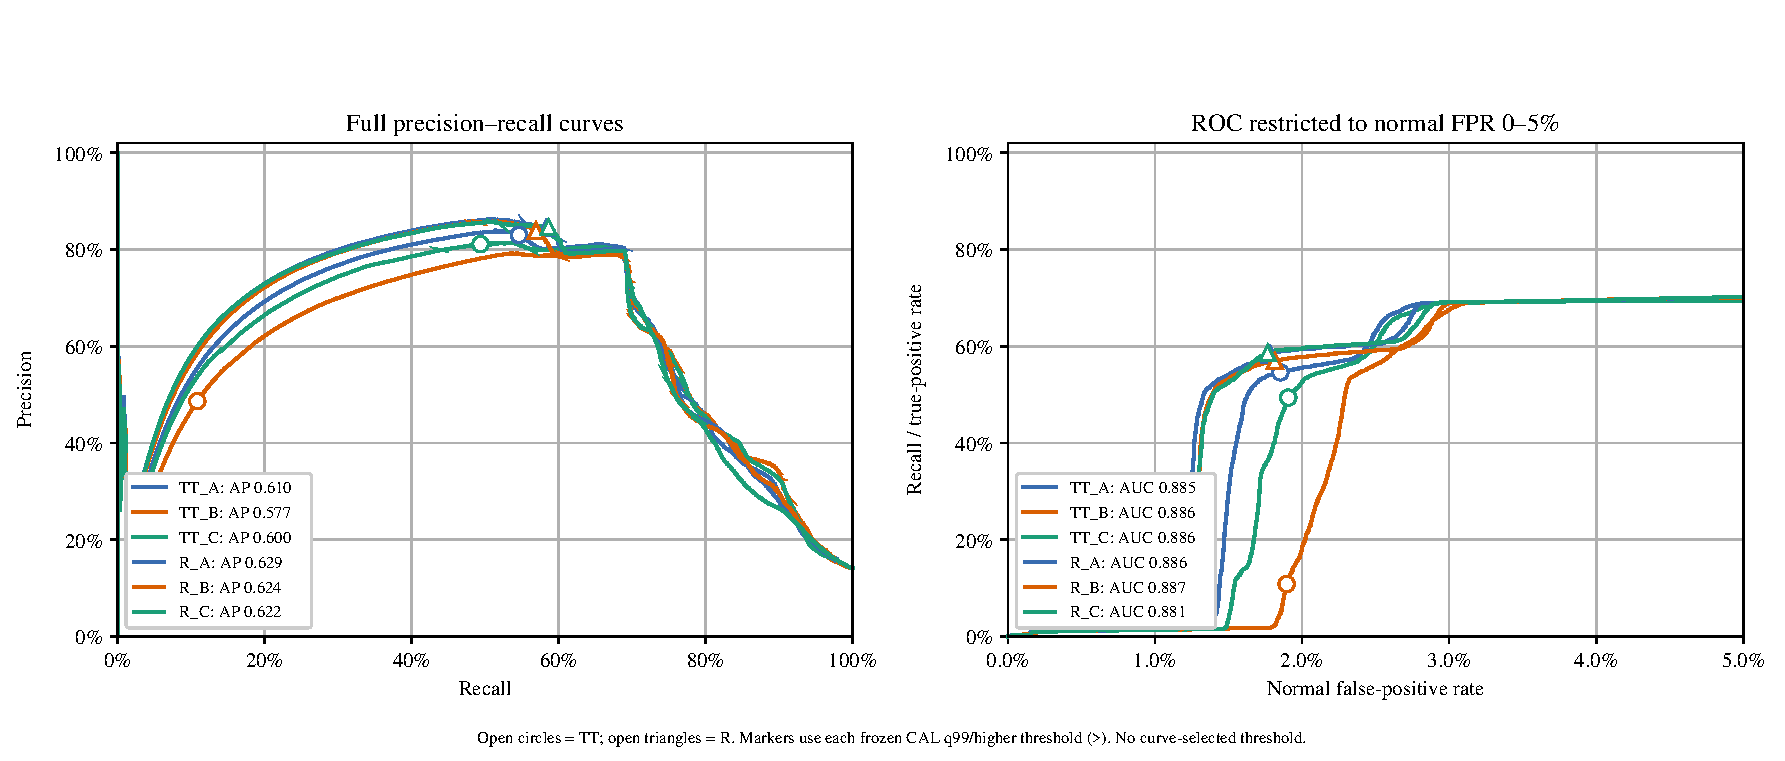
\includegraphics[width=\linewidth,keepaspectratio]{Fig1.pdf}
\caption{Archived SWaT curves for seed 2025. The original calibration
operating points are overlaid on precision-recall and low-FPR ROC
curves. The curves describe threshold variation without selecting a new
threshold.}
\end{figure}

The seed-2025 SWaT TT-B and TT-C ROC-AUCs are 0.885519 and 0.885894.
Their strict recalls at the fixed rule are 10.829\% and 49.358\%, at
normal FPRs of 1.895\% and 1.906\%. Fig. 1 helps explain why full ROC
area alone misses this operating difference. These curves do not identify a unique training or calibration explanation.

\section{Comparison with Existing
Methods}\label{comparison-with-existing-methods}

External comparisons include a plain multilayer perceptron (MLP), CANDI
\citep{candi2026}, and separately archived native TimeRadar head probing
\citep{timeradar2026}. Contrasts within a detector compare update
policies under that detector's protocol. Aligned query indices across
detectors permit descriptive comparisons, with differences in
initialization, standardization, score definition, update rules, and
available observations retained. The shared PSM operating points use an
all-attack calibration set. TimeRadar uses a separate PSM score axis and
calibration archive.

Table 7 presents external comparison permissions.

\begin{longtable}[]{@{}
  >{\raggedright\arraybackslash}p{(\linewidth - 4\tabcolsep) * \real{0.3333}}
  >{\raggedright\arraybackslash}p{(\linewidth - 4\tabcolsep) * \real{0.3333}}
  >{\raggedright\arraybackslash}p{(\linewidth - 4\tabcolsep) * \real{0.3333}}@{}}
\caption{External comparison permissions. Within a row, the
corresponding noU and updating arms use that row's fixed protocol.
Published results are not substituted for missing local
cells.}\tabularnewline
\toprule\noalign{}
\begin{minipage}[b]{\linewidth}\raggedright
Detector
\end{minipage} & \begin{minipage}[b]{\linewidth}\raggedright
Initialization and adaptation permission
\end{minipage} & \begin{minipage}[b]{\linewidth}\raggedright
Readout and comparison scope
\end{minipage} \\
\midrule\noalign{}
\endfirsthead
\toprule\noalign{}
\begin{minipage}[b]{\linewidth}\raggedright
Detector
\end{minipage} & \begin{minipage}[b]{\linewidth}\raggedright
Initialization and adaptation permission
\end{minipage} & \begin{minipage}[b]{\linewidth}\raggedright
Readout and comparison scope
\end{minipage} \\
\midrule\noalign{}
\endhead
\bottomrule\noalign{}
\endlastfoot
LEFT & Task-specific normal-source initialization, native source-prefix
scaler including source validation, matched noU/TT/SS/R & 192-point
full-window offline scores, main SWaT/PSM axes \\
Plain MLP & Task-specific source-FIT-only scaler and source-selected
checkpoint, same legal seed-2025 exposure endpoints for its TT/R &
10-point window reconstruction error at its true endpoint, same point
indices as the main comparison \\
CANDI & Same plain MLP source reference, complete selection and residual
module on chronological unlabeled target FIT, frozen at scoring &
10-point endpoint MSE, local fit-then-freeze protocol rather than native
continuous test-time learning \\
TimeRadar & Author-supplied pretrained state including synthetic anomaly
information in pretraining. Project native-variance noU and decoder-only
TT/SS/R & 100-point endpoint variance, distinct PSM 64,728-point query
axis and separate CAL archive. Historical full-window variants have
different time permissions \\
TSAD-C & Published contaminated-training method. Local scorer and
inference compatibility did not qualify & Local results are NA.
Literature only \\
\end{longtable}

The MLP comparison preserves TT/R's corresponding source and target draw
endpoints using the last 10 points of each authorized training window.
It provides a within-backbone check, not a controlled comparison that
isolates the benefit of LEFT's time-frequency representation. In seed
2025, MLP R improves AP over MLP TT by 0.591 pp on SWaT and 14.077 pp on
PSM. On SWaT, MLP R has 96.090\% confirmed normal FPR and 5 one-to-one
matches versus 21 any-hit events. LEFT R has 1.512\% confirmed normal
FPR and 15 matches. On PSM, MLP R has AP 0.631848 and 3.146\% confirmed
complete-event coverage. LEFT R has AP 0.587891 and 61.901\% coverage at
a higher confirmed normal FPR, 9.677\% versus 0.759\%. These quantities
compare the stored operating points and show why an AP improvement under
replay need not imply better coverage. There are no matched MLP B/C
experiments in this study.

CANDI under the local fit-then-freeze schedule does not materially
improve on its own plain MLP reference at the fixed configuration. SWaT
AP changes from 0.783949 to 0.783885 while the confirmed normal FPR
rises from 96.748\% to 97.356\%. PSM AP is 0.604606 for both after
rounding, with unchanged confirmed event coverage. The comparison does
not measure how CANDI would behave when it can update throughout the
query stream as described in its original setting. The full same-axis
seed-2025 table is in Appendix C.

On the separate TimeRadar head-probing protocol, seed-2025 TT loses AP
relative to noU on both tasks. R versus TT adds 5.426 pp on PSM and
loses 0.590 pp on SWaT. PSM AP recovery does not preserve noU's
sustained coverage. This external reference supports keeping the
conclusions specific to the task and detector. It does not supply
additional matched LEFT seeds. The frozen TimeRadar and TimesFM
comparison and its negative direct complementarity result remain
archival references rather than part of the adaptation claim.

\section{Discussion and Limitations}\label{discussion-and-limitations}

\textbf{What the paired comparison identifies.} Replacing the second
target half-batch with source data changes the training distribution
while preserving the update count, batch size, initialization, and the
first target draw. This makes R\ensuremath{-}TT interpretable as the effect of the
replay policy in a defined experiment. It cannot separate the value of
additional source examples from the effect of giving fewer target
examples the opportunity to influence the detector. R\ensuremath{-}SS and R\ensuremath{-}noU help
interpret those comparisons but cannot by themselves prove that replay
prevented internal forgetting. We did not measure a unique parameter- or
representation-level retention mechanism.

\textbf{Task-dependent exposure effects.} Matching replacement slots
controls their number and location. It leaves donor content and the two
half-batch mixtures different. The abnormal donors come from a small
number of events, and repeated windows can share observations. Donor
pools can differ in the temporal structure of their windows and in the
operational states they represent. SWaT shows smaller AP and coverage
losses with replay at this intervention level, while PSM shows a
different AP response and lower absolute event coverage with replay
under B. These contrasts characterize the fixed donor intervention on
each task. They cannot isolate a universal contamination effect from
differences between the donor pools.

\textbf{Operational meaning.} A detector can assign a better global
ranking yet alarm less often on an event in the selected operating
region. Conversely, when its threshold produces nearly continuous
alarms, any-hit and pooled coverage can appear high regardless of useful
event separation. The original q99 rule gives each arm its own threshold
in score units and does not equalize normal false-positive rates. PSM's
all-attack CAL is a particularly severe limit on operating
interpretations. We retain both rank measures and the fixed rule, with
no query-tuned threshold. The offline full-window LEFT readout and
retrospective location and availability metrics cannot establish online
response times.

\textbf{Generalization and comparison limits.} The primary evidence
spans two exposed public development tasks, each with one initialization
and three adaptation seeds. It supplies no independent site, device,
time split, or pretraining replication. Repeated draws and repeated
scoring of the same events do not widen that support. Plain MLP and
CANDI are available at one seed, with unequal window lengths, scalers,
initializers, and learning permissions relative to LEFT. TimeRadar's
separate protocol and the unavailable local TSAD-C result limit breadth.
All files and claims in this study use public datasets. The observed
protection and parameter trade-offs should not be attributed to a
general guarantee against arbitrary contamination, a new anomaly head,
or transferable time-frequency synergy.

\section{Conclusion}\label{conclusion}

Ordinary target-only updating lowers mean AP relative to noU and SS on
both evaluation tasks, while increasing ROC-AUC on SWaT and confirmed
point coverage on PSM. At matched update and presentation budgets,
replacing half of the target batch with source windows improves AP in
all six within-task seed comparisons and reduces observed false-positive
counts. Confirmed coverage increases relative to TT on SWaT and
decreases on PSM, where all selected calibration points are
attack-labeled. Under the fixed replacement intervention, the AP
advantage from attenuating the B\ensuremath{-}C decrease repeats on SWaT. On PSM, B
raises AP relative to C in both arms. These results characterize the
ranking and detection trade-offs of an established update policy at
defined operating points.

Supplementary appendices give the reproduction protocol, archived result
tables, and computing records.

\section*{Statements and
Declarations}\label{statements-and-declarations}
\addcontentsline{toc}{section}{Statements and Declarations}

\textbf{Data availability.} SWaT benchmark access is provided by
\href{https://www.sutd.edu.sg/itrust/itrust-labs/datasets/dataset-characteristics/swat/}{iTrust},
subject to its access and reuse terms. The
\href{https://github.com/eBay/RANSynCoders/tree/main/data}{eBay PSM
release} provides the public source data. The accompanying supplement
supplies derived result tables and identifies the fixed prepared
representations. Original experiment arrays, model weights and per-point
score caches are held separately. Reviewer access to those assets is
subject to the provider terms and an authorized access arrangement.

\textbf{Code availability.} The supplement identifies the public LEFT
upstream version. The author-hosted adaptation and evaluation archive is
withheld from the anonymous review copy.

Additional author declarations are supplied separately for editorial completion.

\textbf{Writing disclosure.} A large language model assisted with drafting and revising the manuscript and organizing the submission materials. Numerical results were taken from the frozen experiment archive.

\backmatter
\bibliography{references}
\end{document}
